\documentclass[landscape,final]{baposter}

\usepackage[utf8]{inputenc}

\usepackage{times}
\usepackage{calc}
\usepackage{graphicx}
\usepackage{amsmath}
\usepackage{amssymb}
\usepackage{relsize}
\usepackage{multirow}
\usepackage{bm}
\usepackage{array}
\usepackage{bibspacing}

\usepackage{graphicx,capt-of}
\usepackage{multicol}

% \usepackage{pgfbaselayers}
\pgfdeclarelayer{background}
\pgfdeclarelayer{foreground}
\pgfsetlayers{background,main,foreground}

\usepackage{helvet}
%\usepackage{bookman}
\usepackage{palatino}

\renewcommand{\refname}{}
\def \figdir {../figures}

\newcommand{\captionfont}{\footnotesize}

\selectcolormodel{cmyk}

\graphicspath{{images/}}

%%%%%%%%%%%%%%%%%%%%%%%%%%%%%%%%%%%%%%%%%%%%%%%%%%%%%%%%%%%%%%%%%%%%%%%%%%%%%%%%
%%%% Some math symbols used in the text
%%%%%%%%%%%%%%%%%%%%%%%%%%%%%%%%%%%%%%%%%%%%%%%%%%%%%%%%%%%%%%%%%%%%%%%%%%%%%%%%
% Format 
\newcommand{\Matrix}[1]{\begin{bmatrix} #1 \end{bmatrix}}
\newcommand{\Vector}[1]{\Matrix{#1}}
\newcommand*{\SET}[1]  {\ensuremath{\mathcal{#1}}}
\newcommand*{\MAT}[1]  {\ensuremath{\mathbf{#1}}}
\newcommand*{\VEC}[1]  {\ensuremath{\bm{#1}}}
\newcommand*{\CONST}[1]{\ensuremath{\mathit{#1}}}
\newcommand*{\norm}[1]{\mathopen\| #1 \mathclose\|}% use instead of $\|x\|$
\newcommand*{\abs}[1]{\mathopen| #1 \mathclose|}% use instead of $\|x\|$
\newcommand*{\absLR}[1]{\left| #1 \right|}% use instead of $\|x\|$

\def\norm#1{\mathopen\| #1 \mathclose\|}% use instead of $\|x\|$
\newcommand{\normLR}[1]{\left\| #1 \right\|}% use instead of $\|x\|$

%%%%%%%%%%%%%%%%%%%%%%%%%%%%%%%%%%%%%%%%%%%%%%%%%%%%%%%%%%%%%%%%%%%%%%%%%%%%%%%%
% Multicol Settings
%%%%%%%%%%%%%%%%%%%%%%%%%%%%%%%%%%%%%%%%%%%%%%%%%%%%%%%%%%%%%%%%%%%%%%%%%%%%%%%%
\setlength{\columnsep}{0.7em}
\setlength{\columnseprule}{0mm}


%%%%%%%%%%%%%%%%%%%%%%%%%%%%%%%%%%%%%%%%%%%%%%%%%%%%%%%%%%%%%%%%%%%%%%%%%%%%%%%%
% Save space in lists. Use this after the opening of the list
%%%%%%%%%%%%%%%%%%%%%%%%%%%%%%%%%%%%%%%%%%%%%%%%%%%%%%%%%%%%%%%%%%%%%%%%%%%%%%%%
\newcommand{\compresslist}{%
\setlength{\itemsep}{1pt}%
\setlength{\parskip}{0pt}%
\setlength{\parsep}{2pt}%
}

%%%%%%%%%%%%%%%%%%%%%%%%%%%%%%%%%%%%%%%%%%%%%%%%%%%%%%%%%%%%%%%%%%%%%%%%%%%%%%
%%% Begin of Document
%%%%%%%%%%%%%%%%%%%%%%%%%%%%%%%%%%%%%%%%%%%%%%%%%%%%%%%%%%%%%%%%%%%%%%%%%%%%%%
% \renewenvironment{list}{\begin{list}}{\end{list}}
\newenvironment{llist}{\begin{list}{$\bullet$}{\leftmargin=1em \itemindent=0em \parskip=0em \parsep=0pt}}{\end{list}}
\begin{document}
\setlength{\bibspacing}{\baselineskip}



%%%%%%%%%%%%%%%%%%%%%%%%%%%%%%%%%%%%%%%%%%%%%%%%%%%%%%%%%%%%%%%%%%%%%%%%%%%%%%
%%% Here starts the poster
%%%---------------------------------------------------------------------------
%%% Format it to your taste with the options
%%%%%%%%%%%%%%%%%%%%%%%%%%%%%%%%%%%%%%%%%%%%%%%%%%%%%%%%%%%%%%%%%%%%%%%%%%%%%%
\typeout{Poster Starts}
\background{
  \begin{tikzpicture}[remember picture,overlay]%
    \draw (current page.north west)+(-2em,-0em) node[anchor=north west] {\hspace{-2em}\includegraphics[height=1.1\textheight]{silhouettes_background}};
  \end{tikzpicture}%
}
\definecolor{skyblue}{rgb}{0.87,0.9,1}
\definecolor{white}{rgb}{1,1,1}
\definecolor{black}{cmyk}{0,0,0.0,1.0}
\definecolor{darkYellow}{cmyk}{0,0,1.0,0.5}
\definecolor{darkSilver}{cmyk}{0,0,0,0.1}
\definecolor{darkblue}{rgb}{0,0,0.7}
\definecolor{lighterryellow}{cmyk}{0,0,0.2,0.0}
\definecolor{lightyellow}{cmyk}{0,0,0.3,0.0}
\definecolor{lighteryellow}{cmyk}{0,0,0.1,0.0}
\definecolor{lightestyellow}{cmyk}{0,0,0.05,0.0}
\begin{poster}{
  % Show grid to help with alignment
  grid=no,
  % Column spacing
  colspacing=1em,
  % Color style
  bgColorOne=white,
  bgColorTwo=white,
  borderColor=blue,
  headerColorOne=skyblue,
  headerColorTwo=black,
  headerFontColor=black,
  boxColorOne=white,
  boxColorTwo=skyblue,
  % Format of textbox
  textborder=rounded,
  % Format of text header
  eyecatcher=yes,
  headerborder=open,
  headerheight=0.12\textheight,
  headershape=rounded,
  headershade=plain,
  headerfont=\Large\textsf, %Sans Serif
  boxshade=plain,
%  background=shade-tb,
  background=plain,
  linewidth=2pt
  }
  % Eye Catcher
  {
\includegraphics[height=6em]{figures/Bogazici_University_Logo.png}} % No eye catcher for this poster. If an eye catcher is present, the title is centered between eye-catcher and logo.
  % Title
  {\sf \vspace{5pt}%Sans Serif
  %\bf% Serif
  \vspace{-14pt}
  Kinect Assisted Rat Behaviour Analysis for Experiment Automation
}
  % Authors
  {\sf \Large \vspace{5pt} %Sans Serif
  	\textbf{Çağrı Sofuoğlu, İsmet Burak Kadron and Albert Ali Salah}\\
    Department of Computer Engineering, Bo\u{g}azi\c{c}i University, Istanbul, Turkey\\
    \{cagri.sofuoglu, burak.kadron, salah\}@boun.edu.tr

  }
  % University logo
  {
\includegraphics[height=7em]{figures/Bogazici_University_Logo.png}
  }

  \tikzstyle{light shaded}=[top color=baposterBGtwo!30!white,bottom color=baposterBGone!30!white,shading=axis,shading angle=30]

  % Width of left inset image
     \newlength{\leftimgwidth}
     \setlength{\leftimgwidth}{0.78em+8.0em}

%%%%%%%%%%%%%%%%%%%%%%%%%%%%%%%%%%%%%%%%%%%%%%%%%%%%%%%%%%%%%%%%%%%%%%%%%%%%%%
%%% Now define the boxes that make up the poster
%%%---------------------------------------------------------------------------
%%% Each box has a name and can be placed absolutely or relatively.
%%% The only inconvenience is that you can only specify a relative position 
%%% towards an already declared box. So if you have a box attached to the 
%%% bottom, one to the top and a third one which should be in between, you 
%%% have to specify the top and bottom boxes before you specify the middle 
%%% box.
%%%%%%%%%%%%%%%%%%%%%%%%%%%%%%%%%%%%%%%%%%%%%%%%%%%%%%%%%%%%%%%%%%%%%%%%%%%%%%
    %
    % A coloured circle useful as a bullet with an adjustably strong filling
    \newcommand{\colouredcircle}[1]{%
      \tikz{\useasboundingbox (-0.2em,-0.32em) rectangle(0.2em,0.32em); \draw[draw=black,fill=baposterBGone!80!black!#1!white,line width=0.03em] (0,0) circle(0.18em);}}

%%%%%%%%%%%%%%%%%%%%%%%%%%%%%%%%%%%%%%%%%%%%%%%%%%%%%%%%%%%%%%%%%%%%%%%%%%%%%%
  \headerbox{Abstract}{name=abstract,column=0,row=0}{
%%%%%%%%%%%%%%%%%%%%%%%%%%%%%%%%%%%%%%%%%%%%%%%%%%%%%%%%%%%%%%%%%%%%%%%%%%%%%%
\par Video tracking for purposes of behaviour analysis has been used by the researchers
at Psychobiology lab extensively.Video tracking systems enable behavior to be studied in a reliable and consistent way, and over longer time periods than if they are manually recorded.\\ 
\par The system takes an depth data as a digital video signal, cuts out data points that lie outside the range at which the kinect is mounted above the cages, and analyses
the resultant pixels to determine the location of the tracked animals (as well
as other data). Calculations are performed on a series of frames to derive a
set of quantitative descriptors of the animal's movement. \\ 
\par This project aims to provide researchers with a tool to create, repeat and
document animal tracking experiment results in a credible way.
It is meant to provide users with unbiased and structured data to be used to construct behaviour analysis reports.
  }
%%%%%%%%%%%%%%%%%%%%%%%%%%%%%%%%%%%%%%%%%%%%%%%%%%%%%%%%%%%%%%%%%%%%%%%%%%%%%%
  \headerbox{Introduction}{name=intro,column=0,below=abstract}{
%%%%%%%%%%%%%%%%%%%%%%%%%%%%%%%%%%%%%%%%%%%%%%%%%%%%%%%%%%%%%%%%%%%%%%%%%%%%%%
	\par One such system currently in use is EthoVision (from Noldus Information Technology). Which provides detailed analysis tools to researcher when tracking lab rats. But one limitation of the EthoVision is its inability to operate under lowly lit or dark environments. \\
	\par Our project aims to fill the gap in functionality by providing researchers with a robust, easy to use tool that can operate at various physical set-ups under all lighting conditions. to this end Kinect was selected as the ideal sensor due to its ability to operate unhindered under dark lighting conditions.\\

\centering
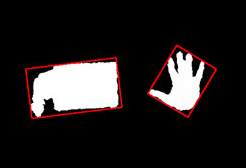
\includegraphics[scale=0.5]{./figures/kinect} 
	\vspace{-12pt}
    \captionof{figure}{Depth data provided by Kinect}
    \label{fig:figure}	
}



%%%%%%%%%%%%%%%%%%%%%%%%%%%%%%%%%%%%%%%%%%%%%%%%%%%%%%%%%%%%%%%%%%%%%%%%%%%%%%
  \headerbox{Implementation}{name=exp,column=1,span=1}{
%%%%%%%%%%%%%%%%%%%%%%%%%%%%%%%%%%%%%%%%%%%%%%%%%%%%%%%%%%%%%%%%%%%%%%%%%%%%%%
	\par The system we developed is going to be used in an experiment where day/light periods are manipulated to observe changes in the rats biological clocks. Thus we decided the depth images provided by the Kinect made the perfect input for the task, as the data is unaffected by any light emission within human visual range.

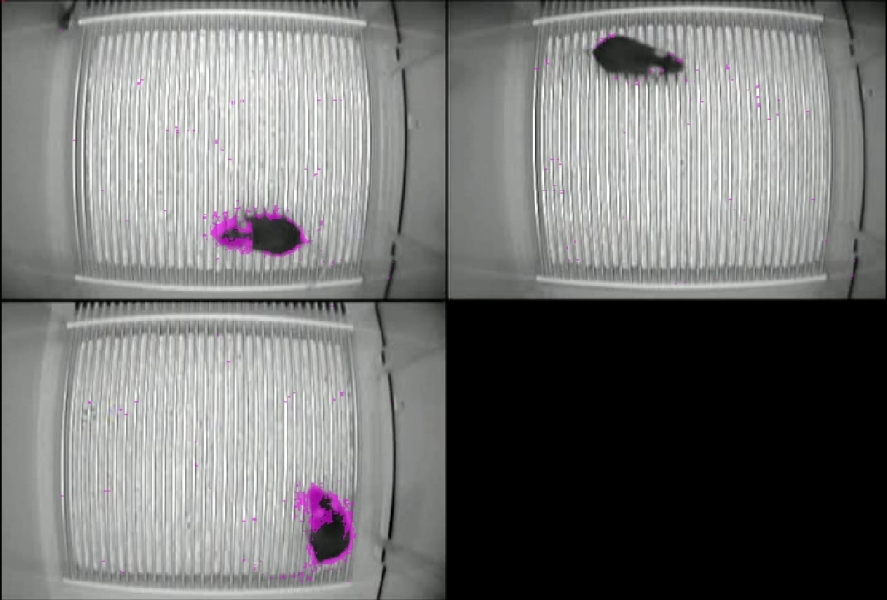
\includegraphics[scale=0.333]{./figures/phy_setup} 
\vspace{-12pt}
    \captionof{figure}{An example set-up with 3 cages.}
    \label{fig:figure}
\vspace{5pt}
	\par The application supports a tracking environment of up to 4 cages, each containing a single subject. The position data gathered is presented to the user in raw form and also in a candle-wick graph describing the speed at which a subject moves within a given period as a indicator of a subject's level of activity. \\
	
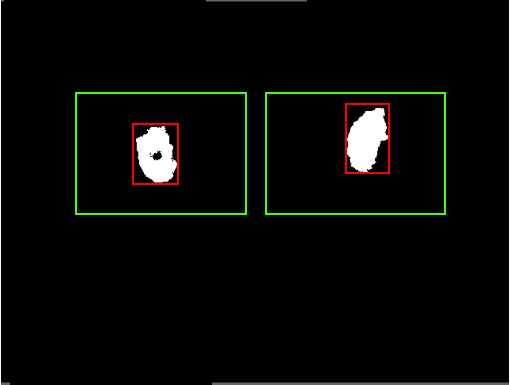
\includegraphics[scale=0.58]{./figures/track} 
\vspace{-16pt}
    \captionof{figure}{Results of tracking with a 2 cage set-up. Cage boundaries are drawn in green and detected rats are marked with a red rectangle }
    \label{fig:figure}
  }
%%%%%%%%%%%%%%%%%%%%%%%%%%%%%%%%%%%%%%%%%%%%%%%%%%%%%%%%%%%%%%%%%%%%%%%%%%%%%%
  \headerbox{Results \& Conclusions}{name=results,column=2}{
%%%%%%%%%%%%%%%%%%%%%%%%%%%%%%%%%%%%%%%%%%%%%%%%%%%%%%%%%%%%%%%%%%%%%%%%%%%%%%
\par We are implemented a system for automatically tracking rat locomotor behaviour for experiment automation.\\
\par We explored the advantages of using Kinect over classical RGB cameras since this approach allows for the system to operate without concerns over lighting conditions. This solution was deemed necessary because the product owners, researchers at the psychobiology lab, require the ability to track and observe subjects in both day and night conditions.\\

\fbox{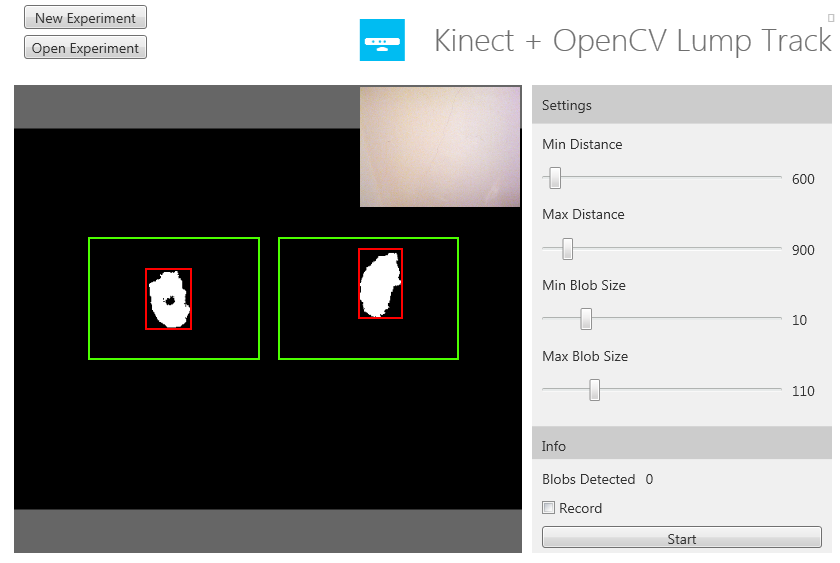
\includegraphics[scale=0.333]{./figures/ui}}
\vspace{-5pt}
    \captionof{figure}{Our current UI.}
    \label{fig:figure}
\vspace{5pt}
\par This project implements behavioural data gathering tool that is as easy to use as possible. For this purpose the tool will as simple a UI as possible. But currently the Psychobiology lab has yet to give us the go ahead for the deployment of our system so the UI has some elements left there for calibration purposes. This unfortunately clutters the UI but will be remedied once the calibrations and on-site long term testing is done. \\

\par All in all, we are happy to say that we have implemented a useful tool which aims help researchers with experiment automation in behavioural analysis studies. As both experiment automation and behavioural analysis are fields that are of much interest both academia and industry, this project has the potential to be further improved upon to create more versatile and precise tools.\\

}%
\headerbox{Acknowledgements}{name=ack,column=3,row=0}{
%%%%%%%%%%%%%%%%%%%%%%%%%%%%%%%%%%%%%%%%%%%%%%%%%%%%%%%%%%%%%%%%%%%%%%%%%%%%%%
%%%%%%%%%%%%%%%%%%%%%%%%%%%%%%%%%%%%%%%%%%%%%%%%%%%%%%%%%%%%%%%%%%%%%%%%%%%%%%
\par We are grateful of members of the Psychobiology Lab who provided us with
an excellent project subject and much needed data and also of Albert Ali Salah who guided us through the project; their hard work and dedication is acknowledged here.
}

%%%%%%%%%%%%%%%%%%%%%%%%%%%%%%%%%%%%%%%%%%%%%%%%%%%%%%%%%%%%%%%%%%%%%%%%%%%%%%
  \headerbox{References}{name=references,column=3,below=ack}{
%%%%%%%%%%%%%%%%%%%%%%%%%%%%%%%%%%%%%%%%%%%%%%%%%%%%%%%%%%%%%%%%%%%%%%%%%%%%%%
\begin{tiny}
	\nocite{Spink2001731,Lind2005123,Cangar200853}
    \setlength{\parskip}{-2mm}
    \bibliographystyle{ieeetr}
    \bibliography{ref}
\end{tiny}
}%

\end{poster}%
%
\end{document}
